\chapter{Aplikacja do wizualizacji danych sensorycznych i komunikacji z robotem}
\label{chap:aplikacja}

W celu ułatwienia procesu strojenia filtrów oraz regulatorów PID stworzono aplikację, którą wyposażono dodatkowo w graficzną reprezentację danych pochodzących z robota w postaci wykresów i wizualizacji 3D. Pozwoliło to wyeliminować problem polegający na konieczności wgrywania za każdym razem nowego programu do mikrokontrolera sterującego robotem w celu zmiany któregokolwiek z parametrów oraz pozwoliło wykryć błędy na etapie implementacji fuzji sygnałów.

%----------------------------------------------------------------------------------------------------------------
\section{Struktura programu}

Główna część programu składa się z zaimplementowanych trzech klas
\begin{itemize}
    \item \texttt{Bluetooth} -- odpowiedzialnej za warstwę komunikacyjną opartą na \texttt{QSerialPort}
    \item \texttt{CommunicationWindow} -- odpowiedzialnej za obsługę interfejsu graficznego okna służącego do nawiązania połączenia z robotem
    \item \texttt{MainWindow} -- odpowiedzialnej za obsługę interfejsu graficznego głównego okna aplikacji
\end{itemize}

Wszystkie wymienione powyżej klasy komunikują się za pomocą mechanizmu slotów i sygnałów, np. klasa \texttt{Bluetooth} po odebraniu i sparsowaniu danych z robota, nadaje sygnał \texttt{Parsed\_frame\_OK()}, który jest powiązany z metodą \texttt{RealTime\_data\_SLOT()} klasy \texttt{MainWindow}, wewnątrz której następuje wyrysowanie danych w oknie głównym aplikacji. 
%----------------------------------------------------------------------------------------------------------------
\section{Funkcjonalności programu}

%----------------------------------------------------------------------------------------------------------------
\subsection{Transmisja dwukierunkowa z robotem}

Za obsługę transmisji odpowiedzialna jest wbudowana w środowisko \texttt{Qt} klasa \texttt{QSerialPort}. Posiada ona szereg metod ułatwiających współpracę z portami dostępnymi na komputerze. Między innymi za pomocą takich metod jak
\begin{itemize}
    \item \texttt{bool setParity(QSerialPort::Parity parity)}
    \item \texttt{bool setBaudRate(qint32 baudRate, QSerialPort::Directions directions = AllDirections)}
    \item \texttt{bool setStopBits(QSerialPort::StopBits stopBits)}
    \item \texttt{bool setDataBits(QSerialPort::DataBits dataBits)}
\end{itemize}
służących do ustawiania parametrów transmisji, oraz
\begin{itemize}
    \item \texttt{virtual void close() override}
    \item \texttt{virtual bool open(QIODevice::OpenMode mode) override}
    \item \texttt{virtual qint64 readData(char *data, qint64 maxSize) override}
    \item \texttt{virtual qint64 writeData(const char *data, qint64 maxSize) override}
\end{itemize}
za pomocą, których zaimplementowano transmisję dwukierunkową z robotem.

Odbieranie i przetwarzanie danych odbywa się na zasadzie przerwania, którego obsługa wykonywana jest po wykryciu sygnału \texttt{readyRead()} generowanego przez obiekt klasy \texttt{QSerialPort} po odebraniu całej ramki danych. Odebrane dane są odpowiednio parsowane i wyświetlane w odpowiednich miejscach.

%----------------------------------------------------------------------------------------------------------------
\subsection{Wyświetlanie danych dotyczących czujnika ruchu i fuzji sygnałów}

Do rysowania wykresów w czasie rzeczywistym, wykorzystano zewnętrzną bibliotekę \texttt{QCustomPlot}. Do funkcji wbudowanych w bibliotekę, które ułatwiają obsługę wykresów należą
\begin{itemize}
    \item zmiana rozdzielczości osi czasu
    \item zmiana zakresów osi X i Y
    \item zmiana kolorów wyświetlanych wykresów
    \item automatycznie skalowanie się zakresu osi w zależności od wyświetlanych danych
\end{itemize}

%----------------------------------------------------------------------------------------------------------------
\subsection{Sterowanie jazdą robota}

Sterowanie jazdą robota, odbywa się za pomocą strzałek wyrysowanych w głównym oknie aplikacji. Po naciśnięciu odpowiedniej strzałki za pomocą myszy, zmienia ona swój kolor na zielony, w celu zasygnalizowania aktualnie zadanego kierunku ruchu. Po naciśnięciu przycisku awaryjnego zmienia on swój stan na wciśnięty i aby go odblokować należy wcisnąć go ponownie. Zmiana prędkości zadanej odbywa się za pomocą suwaka i wyrażona jest w jednostce RPM.          

%----------------------------------------------------------------------------------------------------------------
\section{Interfejs graficzny}

Cały interfejs graficzny został podzielony na dwa główne okna. Pierwsze z nich to okno służące do konfiguracji i połączenia się z portem szeregowym, oraz główne okno, w którym dostępna jest całą reszta funkcjonalności aplikacji. 

%----------------------------------------------------------------------------------------------------------------
\subsection{Okno łączenia}

Okno podzielone jest na trzy główne obszary, których rozmieszczenie zaprezentowano na rysunku \ref{Okno laczenie koncepcja}.
W pierwszym obszarze okna oznaczonym numerem 1 na rysunku \ref{Okno laczenie koncepcja}, znajdują się rozwijane opcje dotyczące portu szeregowego, z którego odczytywane są dane pochodzące z robota w postaci bitowej ramki danych. Do stworzenia rozwijanych list wykorzystano klasę \texttt{QComboBox}.

W obszarze drugim użytkownik aplikacji ma do dyspozycji trzy przyciski:
\begin{itemize}
    \item Szukaj urządzeń -- po naciśnięciu przycisku wyszukiwane są wszystkie porty, a następnie dodawane są do rozwijanej listy
    \item Połącz -- łączy się z portem, który aktualnie został wybrany z rozwijanej listy
    \item Rozłącz -- rozłącza się z aktualnie połączonym portem
\end{itemize}

Obszar trzeci jest konsolą służącą do wyświetlania komunikatów dla użytkownika. Jest to obiekt stworzony za pomocą klasy \texttt{QTextBrowser}. Ponadto w oknie dostępne są dwa przyciski: ,,Anuluj'' oraz ,,Dalej''. Pierwszy z nich kończy działanie aplikacji, natomiast drugi, po poprawnym nawiązaniu połączenia otwiera główne okno aplikacji. Rzeczywisty wygląd okna łączenia z robotem, widoczny jest na zrzucie ekranu \ref{Okno laczenie}.

\begin{figure}[h!]
    \centering
    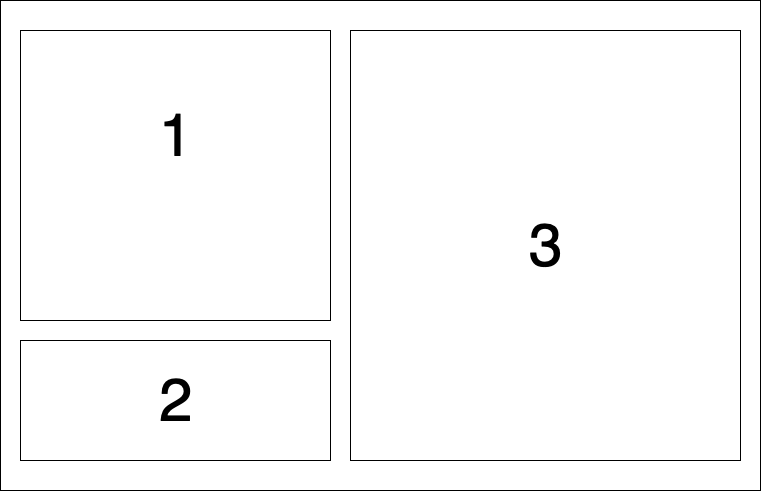
\includegraphics[width=0.75\textwidth]{Rysunki/Rozdzial06/Laczenie_okno_koncepcja.png}
    \caption{Rozmieszczenie elementów w oknie do łączenia z robotem}
    \label{Okno laczenie koncepcja}
\end{figure}

%----------------------------------------------------------------------------------------------------------------
\subsection{Główne okno}

Mając przed oczami główne okno aplikacji w jej lewym górnym rogu oznaczonym jako obszar pierwszy, wyświetla się nazwa aktualnie otwartego portu szeregowego. W prawym, górnym rogu, w obszarze numer dwa dotyczącym zasilania robota, znajduje się aktualne napięcie baterii oraz procentowe określenie stanu naładowania. W zależności od poziomu naładowania wyświetlane są trzy stany naładowania w postaci ikon o kolorze czerwonym (0-24\%), pomarańczowym (25-74\%) oraz zielonym (75-100\%). Do wyświetlania statycznych obiektów graficznych w formacie PNG, wykorzystano klasę \texttt{QPixMap} oraz \texttt{QLabel}.

W trzecim obszarze znajduje się obiekt graficzny stworzony z wykorzystaniem klasy \texttt{QTabWidget}. Za jego pomocą możemy definiować zakładki, z których każda jest oddzielnym oknem, w którym możemy umieszczać inne obiekty graficzne. Na potrzeby aplikacji stworzono pięć zakładek:
\begin{itemize}
    \item Żyroskop -- wykres z aktualnymi odczytami dla żyroskopu w osiach XYZ wyrażonymi w $^o/s$
    \item Akcelerometr -- wykres z aktualnymi odczytami dla akcelerometru w osiach XYZ wyrażonymi w $g$
    \item Magnetometr -- wykres z aktualnymi odczytami dla magnetometru w osiach XYZ wyrażonymi w $\mu T$
    \item Fuzja pomiarów -- wykres z aktualnymi wartościami obliczonymi przez aktualnie wybrany algorytm fuzji sygnałów wyrażonymi w kątach RPY
    \item Panel sterowania -- aktualne nastawy regulatorów PID oraz możliwość ich edycji, podgląd zmiennych odbieranych z robota, możliwość zmiany parametrów związanych z algorytmami fuzji sygnałów, wybranie filtru aktualnie biorącego udział w algorytmie sterowania
\end{itemize}

W obszarze numer cztery, użytkownik ma podgląd na aktualną orientację robota wyświetlaną w środowisku \texttt{OpenGL}, na podstawie odebranych kątów RPY obliczonych przez mikrokontroler robota. Zaraz poniżej w obszarze numer pięć użytkownik ma dostęp do panelu sterowania za pomocą, którego możliwe jest wymuszenie poruszania się robota w przód-tył oraz prawo-lewo, za pomocą czterech strzałek. Dodatkowo stworzono przycisk awaryjny, który po naciśnięciu przesyła do robota informację o tym, aby wyłączył napęd. Tak, aby możliwe było zmienianie aktualnej prędkości zadanej robota, wykorzystano do tego suwak stworzony za pomocą klasy \texttt{QSlider}, oraz podgląd za pomocą klasy \texttt{QLCDNumber}. Rzeczywisty wygląd okna zobaczyć, można na zrzutach ekranu, \ref{Okno panel}, \ref{Okno fuzja}, \ref{Okno zyro}.

Na samym dole okna zdefiniowano przyciski z następującymi funkcjami:
\begin{itemize}
    \item Stop -- zatrzymuje rysowanie wykresu
    \item Resetuj -- czyści wykres
    \item Wyśrodkuj -- maksymalizuje okno aplikacji po ręcznej zmianie jego wymiarów za pomocą myszki
    \item Rozłącz -- rozłącza aktualny port i przechodzi do okna łączenia
    \item Wyślij -- wysyła ramkę danych do robota, np. po zmianie nastaw PID przez użytkownika
    \item Zakończ -- kończy działanie aplikacji
\end{itemize}

\begin{figure}[h!]
    \centering
    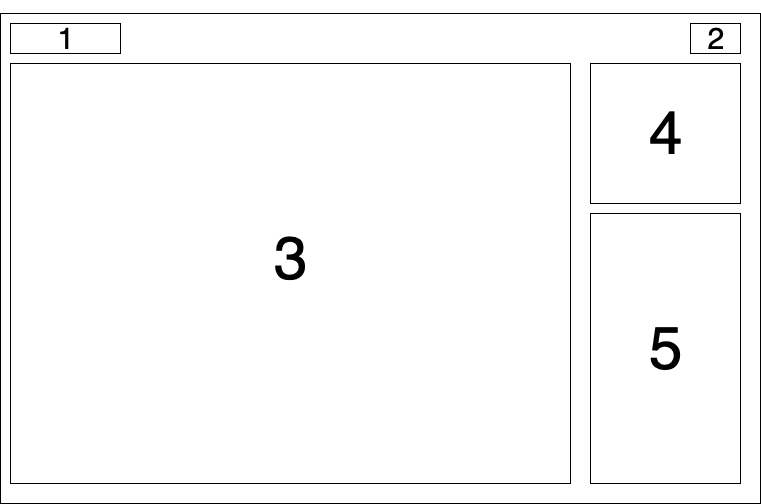
\includegraphics[width=0.75\textwidth]{Rysunki/Rozdzial06/Glowne_okno_koncepcja.png}
    \caption{Okno główne aplikacji}
    \label{Okno glowne}
\end{figure}

\newpage
%----------------------------------------------------------------------------------------------------------------
\section{Zrzuty ekranu}

\begin{figure}[h!]
    \centering
    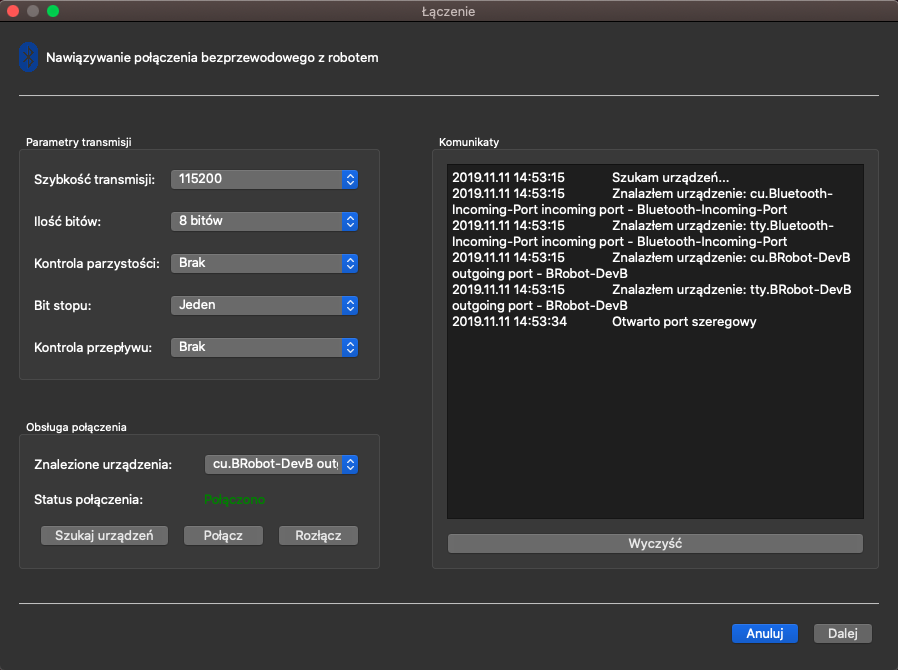
\includegraphics[width=1\textwidth]{Rysunki/Rozdzial06/Okno_laczenia.png}
    \caption{Okno do łączenia się z robotem}
    \label{Okno laczenie}
\end{figure}

\begin{figure}[h!]
    \centering
    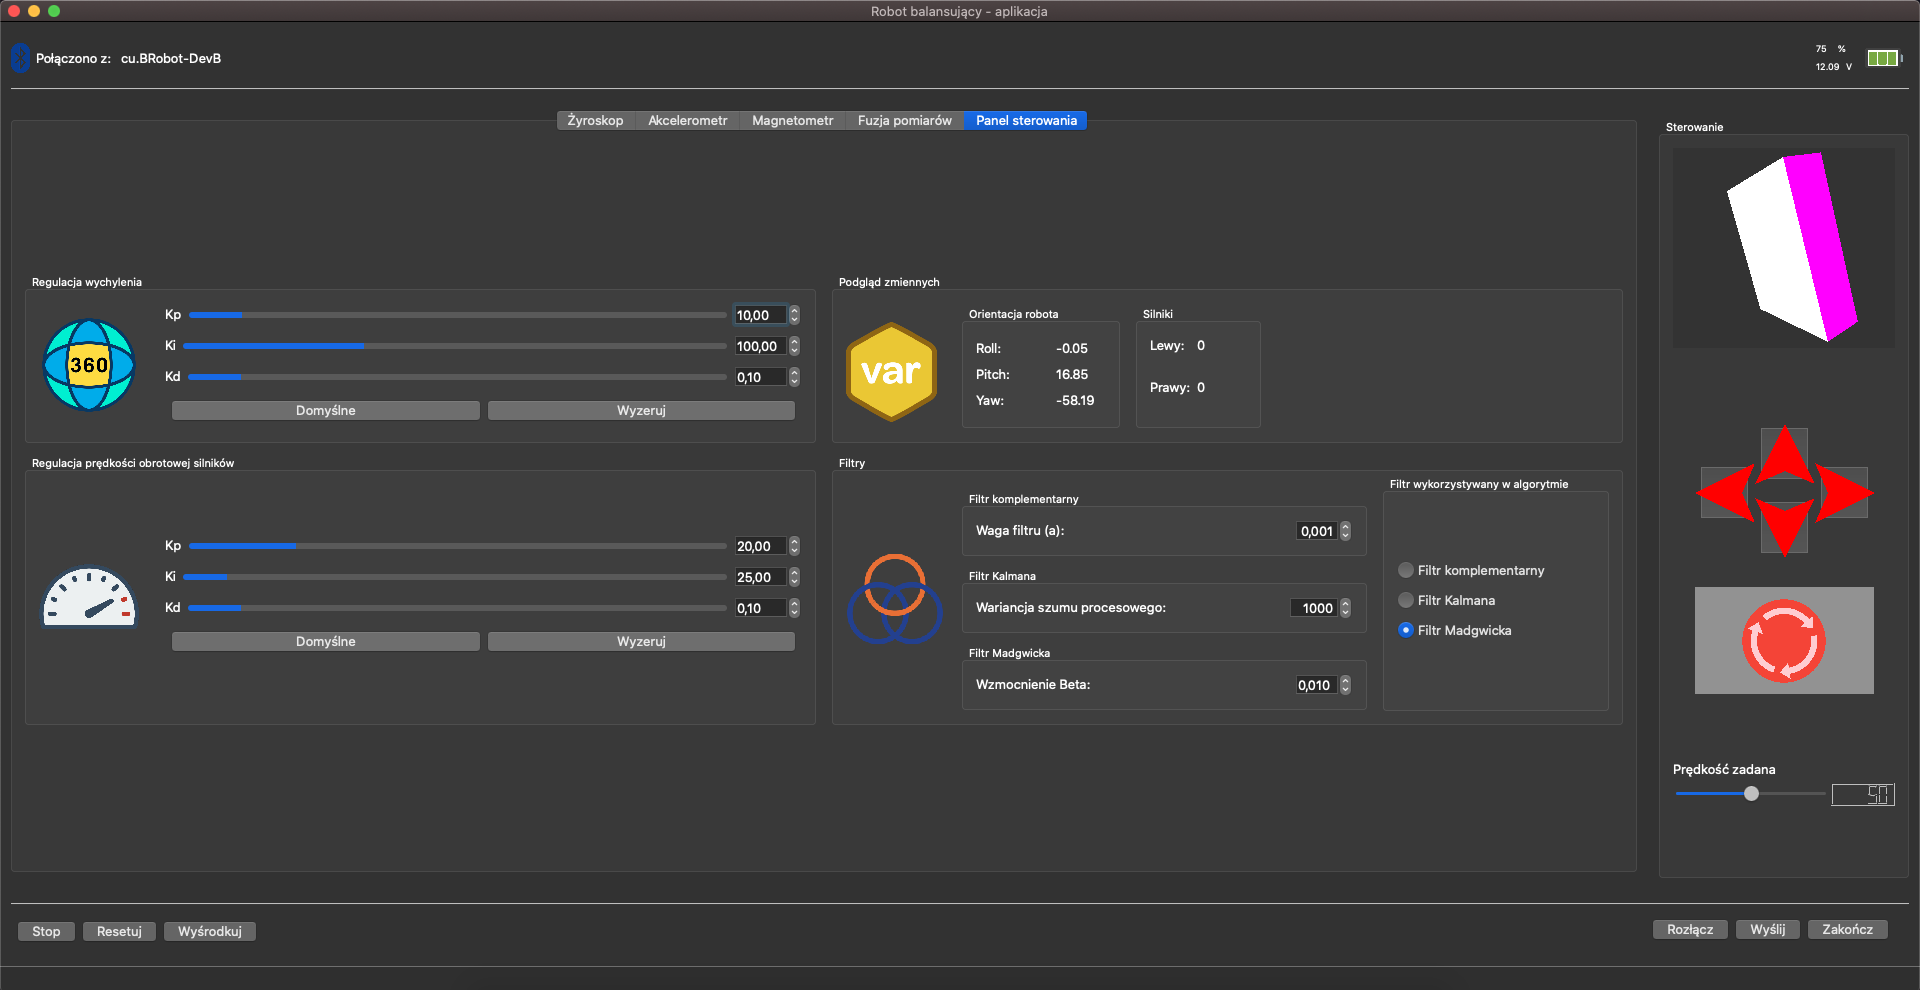
\includegraphics[width=1\textwidth]{Rysunki/Rozdzial06/Panel_sterowania.png}
    \caption{Okno z panelem operatorskim}
    \label{Okno panel}
\end{figure}

\begin{figure}[h!]
    \centering
    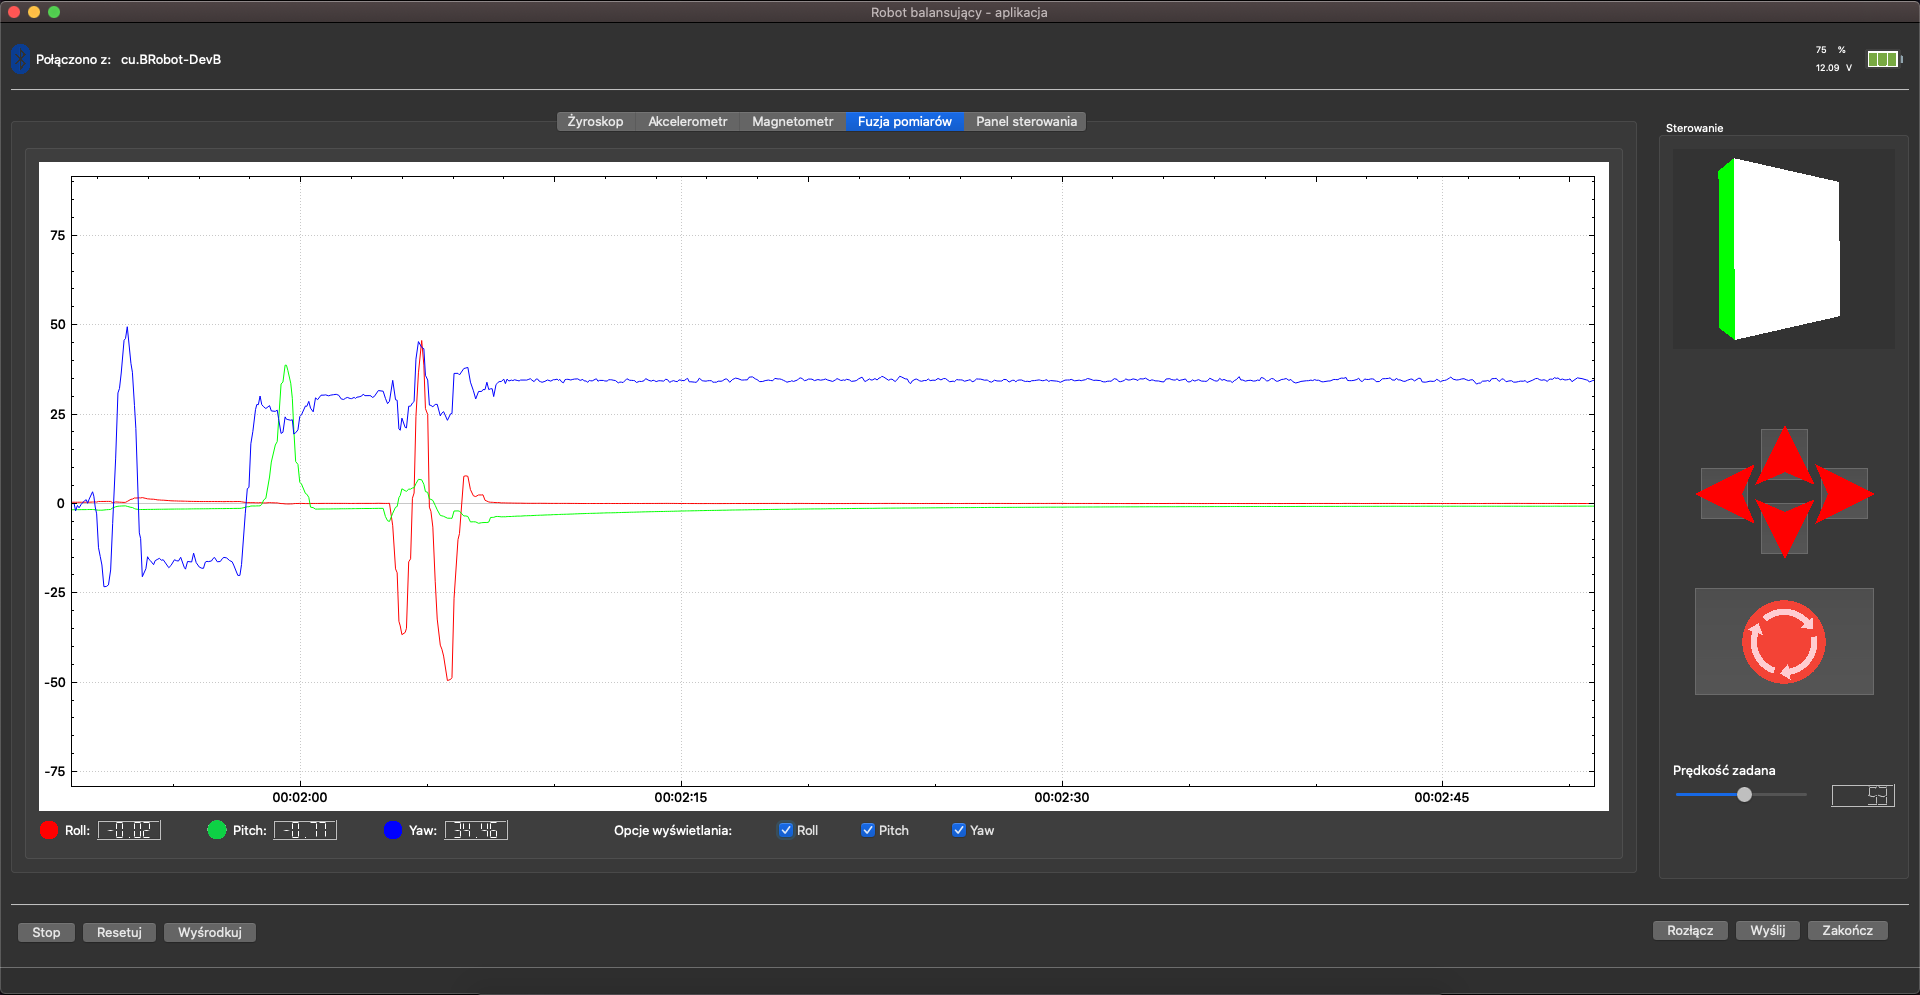
\includegraphics[width=1\textwidth]{Rysunki/Rozdzial06/Fuzja.png}
    \caption{Okno z wykresami dotyczącymi fuzji sygnałów}
    \label{Okno fuzja}
\end{figure}

\begin{figure}[h!]
    \centering
    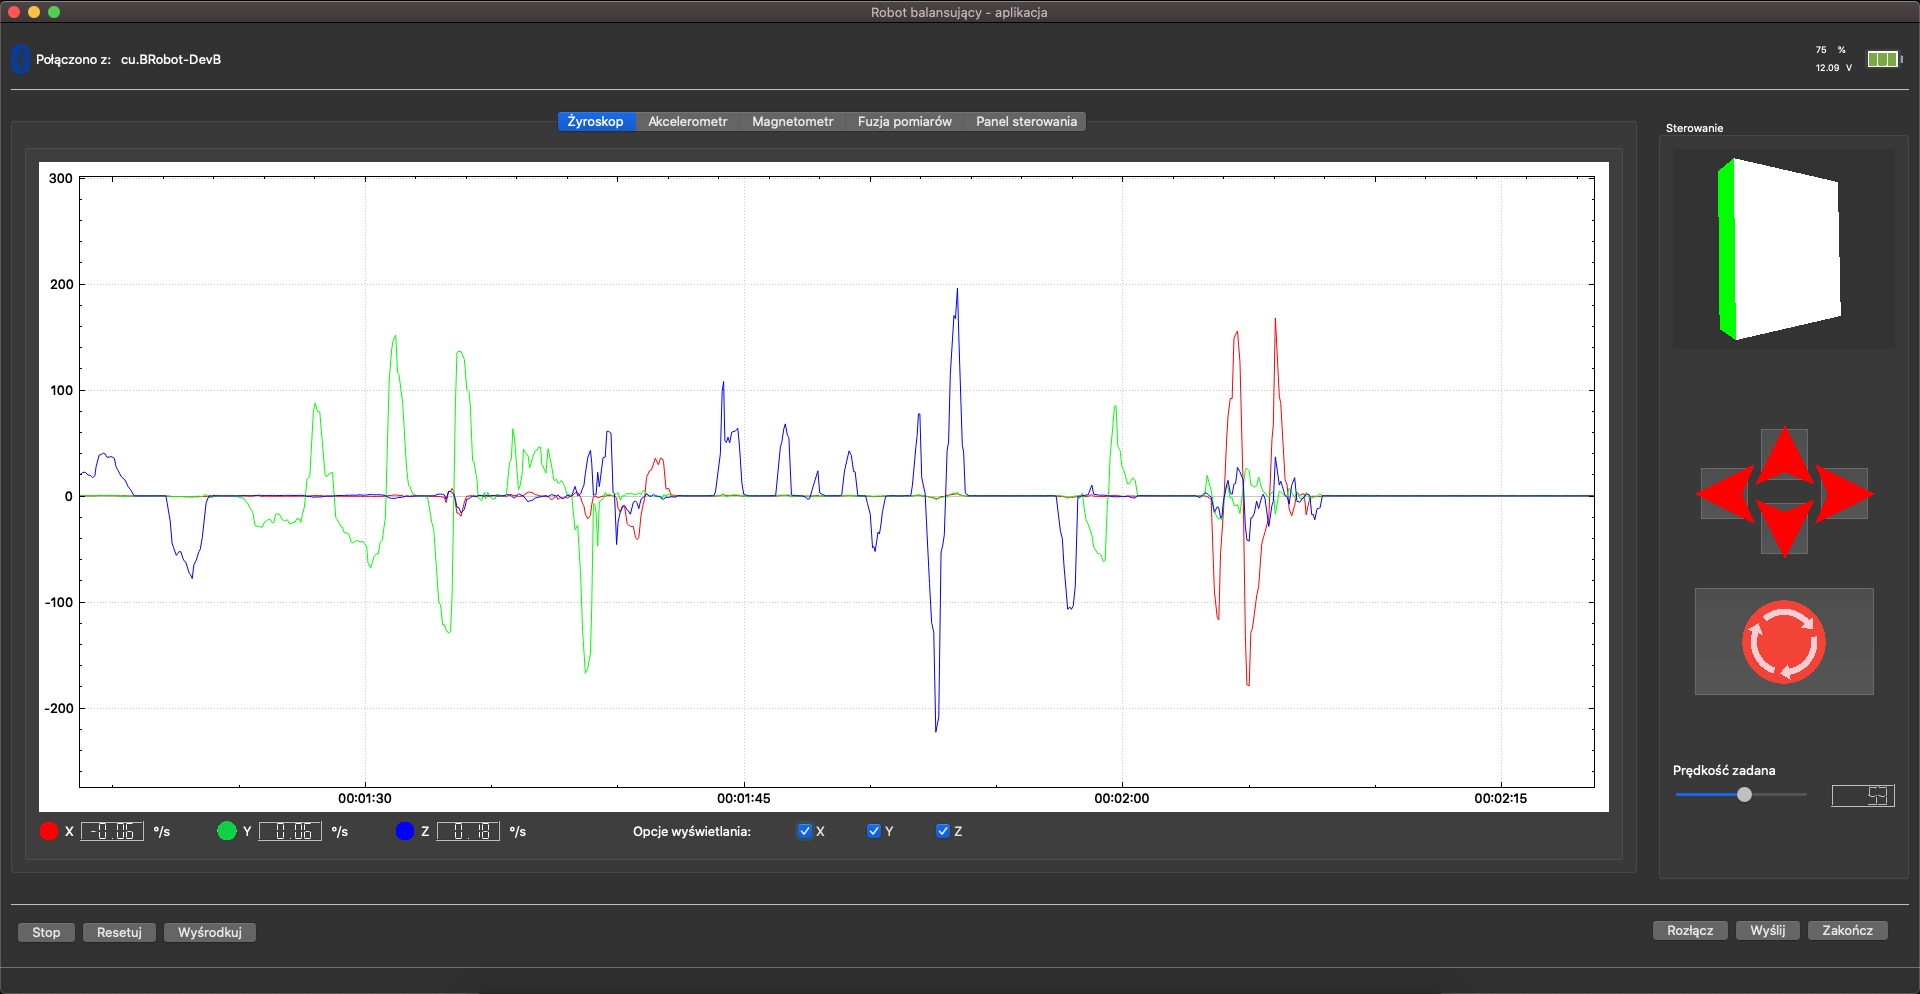
\includegraphics[width=1\textwidth]{Rysunki/Rozdzial06/Zyro.png}
    \caption{Okno z wykresami dotyczącymi żyroskopu}
    \label{Okno zyro}
\end{figure}

%----------------------------------------------------------------------------------------------------------------